\documentclass[11pt,letterpaper, onecolumn]{exam}
\usepackage{amsmath}
\usepackage{amssymb}
\usepackage{units}
\usepackage{xcolor}
\usepackage{color}
\usepackage{graphicx}
\usepackage{booktabs}
\usepackage{mhchem}
\usepackage{subfig}
\usepackage{cancel}
\usepackage{listings}
\usepackage{wrapfig}
\usepackage{lastpage}
\usepackage{float}
\usepackage{caption}
\usepackage{multirow}
\usepackage{tikz}
\usepackage{lipsum}
\setlength{\parindent}{0em}
\allowdisplaybreaks
\setcounter{section}{2} % Set this to match the problem numbers

%New colors defined below
\definecolor{codegreen}{rgb}{0,0.6,0}
\definecolor{codegray}{rgb}{0.5,0.5,0.5}
\definecolor{codepurple}{rgb}{0.58,0,0.82}
\definecolor{backcolour}{rgb}{0.95,0.95,0.92}
\definecolor{green}{rgb}{0.71, 0.95, 0.65}

%Code listing style named "mystyle"
\lstdefinestyle{mystyle}{
  backgroundcolor=\color{backcolour},   commentstyle=\color{codegreen},
  keywordstyle=\color{magenta},
  numberstyle=\tiny\color{codegray},
  stringstyle=\color{codepurple},
  basicstyle=\ttfamily\footnotesize,
  breakatwhitespace=false,         
  breaklines=true,                 
  captionpos=b,                    
  keepspaces=true,                 
  numbers=left,                    
  numbersep=5pt,                  
  showspaces=false,                
  showstringspaces=false,
  showtabs=false,                  
  tabsize=2
}

%"mystyle" code listing set
\lstset{style=mystyle}


\lhead{YOUR NAME\\}
\rhead{CLASS NUMBER: Problem Set \#N\\}
\chead{\hline} % Un-comment to draw line below header
\thispagestyle{empty}   %For removing header/footer from page 1
\cfoot{\hline \\ Page \thepage\ of \pageref{LastPage}}

\begin{document}

\begingroup  
    \centering
    \LARGE CLASS NUMBER: CLASS NAME\\
    \LARGE Problem Set \#N\\[0.5em]
    \large Thursday, September 1, 2022\par
    \large YOUR NAME\par
    \large email@berkeley.edu\par
\endgroup
\rule{\textwidth}{0.4pt}
\pointsdroppedatright   %Self-explanatory
\printanswers


%%%%%%%%%%%%% QUESTION 1 %%%%%%%%%%%%%%%%
\section{Numbered First Question}
\lipsum[2]

\begin{gather*}
    \frac{dC}{dt} + 0.06 C = 0 \\
    C(t=0) = 10^7 \, \mathrm{parts}/\mathrm{m^3} \\
    \Delta t = 1 \, \mathrm{week}
\end{gather*}

\subsection{Numbered First Sub-Question}
\lipsum[5]

\begin{gather}
    y_{n+1} = y_n + \frac{1}{6} \Delta x \left( K_1 + 2 K_2 + 2 K_3 + K_4 \right)
\end{gather}

\lipsum[3]

\begin{figure}[H]
    \centering
    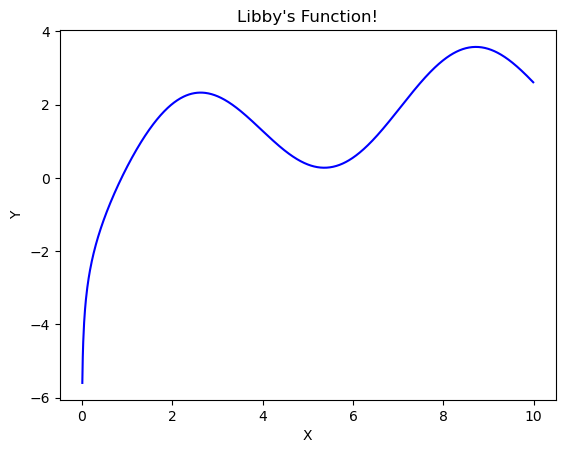
\includegraphics[width = 0.65 \textwidth]{example_figure.png}
    \caption{A caption about your figure.}
    \label{fig:example_fig}
\end{figure}

As shown in Figure \ref{fig:example_fig}, \lipsum[3] 

\begin{center}
\begin{tabular}{|| c || c | c | c | c | c | c ||} 
\hline \hline
\toprule
     A &  B &  C &  D &  E &  F & G \\ \hline \hline
\midrule
   \multirow{2}{*}{Example Multirow} &  \multicolumn{6}{ c ||}{Multicolumns} \\ \cline{2-7}
    &  1 &  2 &     3 &  4 &  5 & 6 \\ \hline
   Example 2 &  7 &   8 &     9 &  10 &  11 & 12 \\ \hline \hline
\bottomrule
\end{tabular}
\end{center}

%%%%%%%%%% Code %%%%%%%%%%%%%%
\clearpage
\section*{Python Code for Problem \#N}

\lstinputlisting[language=Python]{example_code.py}
    
%%%%%%%%%% End Matter %%%%%%%%%%%%%%
\end{document}